% for sublime text 3
%!TEX root = diss.tex

\chapter{Lexical Cohesion Graph}
\label{ch:lex-graph}

\section{Introduction}
\label{sec:introduction}
A \mbox{well-written} is more than a random collection of sentences: it shows connectedness. 
The concept of coherence is based on cohesive semantic relations connecting elements of a text. 
Cohesive relations are expressed through grammar and the vocabulary of a language. 
The former is referred to as \emph{grammatical coherence}, the latter as \emph{lexical coherence}\ \cite{halliday76}. 
Grammatical coherence encompasses coreference, substitution, ellipsis, etc. 
For instance, the entity graph model is mainly based on entities that are defined as coreferent mentions in a document.  
Lexical cohesion is one of the important cohesion-creating devices in texts \cite{hoey91} and comprises one of the semantic connections among words of a text. 
In this chapter, we measure text coherence by modeling \emph{lexical cohesion} that is 
built on semantic relations between words of sentences. 


The basis of lexical cohesion is in fact extended to any pair of lexical items that stand next to each other in some recognizable lexicosemantic relation \cite{sandres06}.


\newcite{stotesbury93} categorize lexical relations as follows:
\begin{itemize}
\item Simple lexical repetition: which means lexical items appear in an identical form e.g.,\ debate (sg.) -- debates (pl.)
\item Complex repetition: covers the cases sharing a lexical morpheme (e.g. history -- historian); antonym formed by affixes (e.g. significant -- insignificant)
\item Simple lexical paraphrase: this can be mutual or partial. 
Partial paraphrase would be for example reference made by a paraphrase, historian, to a person whose name was mentioned earlier. 
\item Complex paraphrase: this covers three different cases: 
\begin{itemize}
    \item antonyms that are not formed with affixes (e.g. willing -- reluctant)
    \item the link triangle comes into play when there are two repetitive links already identified. 
    For example the relation between history and historian, and historian is related to scholar. 
    \item third case occurs when one of the two links is missing but could imagine to exist in a particular context. 
\end{itemize} 

\item repetition that happens when a word of a sentence is repeated in another sentence;

\item synonymy that happens when a word of a sentence means exactly or nearly the same as a word in another sentence. 
For example, verbs ``buy'' and ``purchase'' have synonymy relation;  

\item hyperonymy that shows the relationship between a generic word (hypernym) in a sentence and a specific instance of it (hyponym) in another sentence. 
For example, words ``red'', ``blue'' and ``color'' are semantically related because they have hyperonymy relation;

\item meronymy that happens when a word of a sentence is a constituent part of, or a member of a concept that is mentioned by a word in another sentence. 
For example, finger and hand have the meronymy relations because a finger is part of a hand;

\item ...
\end{itemize}

\cite{halliday76} explain that there is coherence between any pair of lexical items that stand to each other in some lexico-semantic relation, regardless of the relation type. 
Based on \cite{halliday76}, for the texture purposes it is only necessary to recognize semantically related lexical items. 
The other important point is that lexical items should not necessarily have the same reference \cite{halliday76}. 
Consider the following example: 

\begin{quote}
\emph{Why does the little boy wriggle all the time? Girls don't.}
\end{quote}

In this example the lexical items \emph{boy}\ and \emph{girls}\ are semantically related and make these two sentences related.  
They do not refer to the same entity, though. 

In order to recognize lexical semantic relations between words, we need to employ some world knowledge. 
One way to do this, is using a resources such as WordNet \cite{fellbaum98} or Freebase \cite{bollacker08}.  
This way is expensive in terms of determining the best resource.  
WordNet lacks broad coverage in particular with proper names, Freebase is restricted to nominal concepts and entities. 
In addition, they are rarely available for other languages than English.
If they are available, almost none of them come close to WordNet's size and coverage on English. 

The other way is to use word embeddings that are train a large corpora. 
Embedding representations of words let us efficiently compute semantic relations among lexical items in the vector space. 
Words that are semantically related in the text space, their embeddings are similar to each other in the vector space. 
These vectors can be easily trained for any language if a large corpus of documents on the language is available. 
The main advantage of word embeddings is that semantic relations between words can simply be computed by the cosine function and the semantic relations between words is relative.  
So we use word embeddings to check the existence of a semantic relations between two words. 

In the following example the sentences are connected because of the semantic relation between \emph{king}\ and \emph{queen}\ which can be induced by word embedding models \cite{mikolov13c,pennington14}.

\begin{quote}
  \emph{\ldots The king was in his counting-house, counting out his money,\\ 
    The queen was in the parlour, eating bread and honey.} 
\end{quote}


Since graph representations of entity-based relations across sentences in a document have been shown useful for modeling coherence, we propose to encode lexical relations among sentences in a document by a graph as well. 
We name our mode lexical coherence graph (LCG) that encodes if semantic relations between words of sentences.  
Therefore, the main contribution of this chapter is that we extends semantic relations between sentences from entity-based relations to lexical-based relations using word embeddings and propose a new approach for encoding these relations via graphs. 

Given lexical coherence graphs of documents in a dataset, similar to the previous chapter, we apply a subgraph mining algorithm to mine all patterns occurring in these graphs. 
We take subgraphs as coherence patterns and use their frequency as features representing the connectivity of the graph and, hence, the coherence of a document. 
Although using the frequency of subgraphs of the lexical coherence graph encodes coherence features well, the subgraph frequency method, in general, is suffering from a sparsity problem when the size of subgraphs increases. 
Large subgraphs capture more structural information, but they occur rarely in graph representations of documents.  
We resolve this sparsity issue by adapting \mbox{Kneser-Ney} smoothing \cite{heafield13} to smooth subgraph frequencies. 
We estimate the probability of unseen subgraphs with respect to similar subgraphs (in terms of connectivity style) that are seen before.  
This estimation enables our model to measure the coherence of a document even when its corresponding graph representation does not contain large subgraphs. 
If the unseen coherence pattern is similar to seen ones, smoothing gives it closer
probability to seen coherence patterns in comparison to dissimilar
unseen ones. 


In order to evaluate our model, we apply our coherence model to readability assessment task as an important task for coherence evaluation. 
The goal of this task is to rank documents with respects to their readability. 
The more coherent a text, the faster to read and easier to understand it is. 
We evaluate our LCG model on the two readability datasets provided by \newcite{pitler08} and \newcite{declercq14}. 
The results indicate that the LCG model outperforms \mbox{state-of-the-art} systems. 
By applying \mbox{Kneser-Ney} smoothing we solve the sparsity problem. 
Smoothing allows us to exploit the high informativity of large subgraphs which leads to new \mbox{state-of-the-art} results in readability assessment.
% Other coherence models \cite{barzilay08,guinaudeau13,mesgar14} are also evaluated on this
% task.
% \newcite{pitler08} use the entity grid \cite{barzilay08} to capture the coherence of a text for readability assessment. 
% \newcite{mesgar15} extend the entity graph \cite{guinaudeau13} as coherence model to measure the readability of texts. They encode coherence as a vector of
% frequencies of subgraphs of the graph representation of a text. 
% We build upon their method and represent the connectivity of sentences in our LCG model by a vector of frequencies of subgraphs.

We summarize the contributions of this chapter as follows:

\begin{itemize}

  \item Proposing a new \mbox{graph-based} representation of lexical semantic relations across sentences,

  \item Adapting \mbox{Kneser-Ney} smoothing approach in order to solve the sparsity problem in frequency of large coherence patterns,  

  \item Evaluating the model on two readability datasets \newcite{pitler08} and \newcite{declercq14}

\end{itemize}


\section{Lexical Cohesion Graph (LCG)}
\label{sec:lexical_coherence_graph}
In this section, we introduce a new graph representation of lexical semantic relations  across sentences in a document. 
We extract all occurring subgraphs in lexical graphs of documents in a dataset to obtain coherence patterns.  
Then we compute frequencies of coherence patterns in a lexical graph of a document to capture the connectivity style of the graph and therefore the perceived coherence of the document. 

\subsection{Graph Model} 
We model semantic relations between sentences by a graph
$G = < V, E > $ where $V$ is a set of nodes representing sentences in a document, and
$E$ is a set of directed edges. 
An edge between two nodes represents existence of a lexical semantic relation between the sentences and the direction of the edge indicates the sentence order in the document.   
Two sentences are semantically connected if there is at least one strong semantic relation between words of the sentences. 
Semantic relations between words are modeled by their corresponding pre-trained word embeddings \cite{pennington14}. 
Given word vectors $v_a$ for word $a$ of sentence $A$ and $v_b$ for word $b$ of sentence $B$, the cosine similarity value, $cos(v_a,v_b)$, between these two word vectors is a measure of semantic connectivity of words $a$ and $b$. 
The range of $cos(v_a,v_b)$ is between $\lbrace -1, +1 \rbrace$. 
One interpretation of cosine is the normalized correlation coefficient, which states how well its two input words are semantically correlated \cite{manning99}. 
The absolute value of cosine, $|cos(v_a,v_b)|$, encodes how strongly two words are
connected.

The connection between sentences is obtained from connections between their words (Figure \ref{f:wrd_rel}). 
Assume sentence $A$ precedes sentence $B$, each word $b$ of sentence $B$ is connected with word $a^\ast$ of $A$, where

\begin{equation*}
a^\ast= \argmax_{a\in A}cos(b,a)
\end{equation*}

\begin{figure}[!ht]
\centering
\small

\begin{tabular}{c}
\begin{tikzpicture}[shorten >=1pt,->,scale=0.62]

     \tikzstyle{word}=[circle,thick,draw=black!75,fill=black!10,minimum size=2mm]
     \tikzstyle{sent}=[ellipse, draw, minimum height=1.5cm]
        \tikzstyle{edge}=[draw, dashed,-]
       \begin{scope}  
         \node [word] (w1) at (0,0) {\tiny{$v_1$}};
         \node [word] (w2) at (2,0) {\tiny{$v_2$}};
         \node [word] (w3) at (4,0) {\tiny{$v_3$}}; 
          \node[sent, minimum width=4cm]  (A) at (2,0) {};         
    
    
         \node [word] (w4) at (8,0) {\tiny{$v_4$}}; 
         \node [word] (w5) at (10,0) {\tiny{$v_5$}}; 
         \node[sent, minimum width=3cm ] (B) at (9,0) {};         

         
         
         \path[edge , bend right=60] (w4) edge [above] node[font=\tiny] {} (w1);
         \path[edge, bend right=60, solid] (w4) edge [above] node[font=\tiny] {} (w2);
         \path[edge, bend right=60] (w4) edge [above] node[font=\tiny] {} (w3);
          
        
         \path[edge ,bend left=60] (w5) edge [above] node[font=\tiny] {} (w1);
         \path[edge,bend left=60] (w5) edge [above] node[font=\tiny] {} (w2);
         \path[edge,bend left=60, solid] (w5) edge [above] node[font=\tiny] {} (w3);
        \end{scope}        
      \end{tikzpicture}
\end{tabular}
\caption{Sentence A with three word vectors $\lbrace v_1,v_2,v_3 \rbrace$ and
  sentence B with two word vectors $\lbrace v_4, v_5 \rbrace$. 
  $v_4$ has the maximum similarity with $v_2$ and $v_5$ with $v_3$.} 
\label{f:wrd_rel}
\end{figure}

We consider $|cos(b,a^\ast)|$ as the weight of the edge that connects word $b$ of sentence $B$ to word $a^\ast$ of sentence $A$. 
We connect each word of $B$ with the most semantically related word of $A$. 
Then from all connections between the words of sentences $A$ and $B$, the connection with the maximum weight among the words of $B$ is selected to connect these two sentences (Figure \ref{f:sent_rel}) in lexical graph. 
We prune all edges whose weights are less than a threshold.  
We use threshold because the resulting graph is complete, we filter
out edges whose weights are below a threshold. 
\begin{figure}[!ht]
\centering
\small

\begin{tabular}{c}
\begin{tikzpicture}[shorten >=1pt,->,scale=0.62]

     \tikzstyle{word}=[circle,thick,draw=black!75,fill=black!10,minimum size=2mm]
      \tikzstyle{sent}=[ellipse, draw, minimum height=1.5cm]
        \tikzstyle{edge}=[draw, dashed,-]
       \begin{scope}  
         \node [word] (w1) at (0,0) {\tiny{$v_1$}};
         \node [word] (w2) at (2,0) {\tiny{$v_2$}};
         \node [word] (w3) at (4,0) {\tiny{$v_3$}}; 
          \node[sent, minimum width=4cm]  (A) at (2,0) {};         
    
    
         \node [word] (w4) at (8,0) {\tiny{$v_4$}}; 
         \node [word] (w5) at (10,0) {\tiny{$v_5$}}; 
         \node[sent, minimum width=3cm ] (B) at (9,0) {};         

          
          \path[edge, bend right=60] (w4) edge  (w2);
          
          \path[edge, bend left=60, thick] (w5) edge (w3);
      \end{scope}        
  \end{tikzpicture}

\\
(a)

\\
      
  \begin{tikzpicture}[shorten >=1pt,->,scale=0.62]

     \tikzstyle{word}=[circle,thick,draw=black!75,fill=black!10,minimum size=2mm]
      \tikzstyle{sent}=[ellipse, draw, minimum height=1.5cm]
      \tikzstyle{edge}=[draw]
       \begin{scope}  
         \node [word] (w1) at (0,0) {\tiny{$v_1$}};
         \node [word] (w2) at (2,0) {\tiny{$v_2$}};
         \node [word] (w3) at (4,0) {\tiny{$v_3$}}; 
          \node[sent, minimum width=4cm]  (A) at (2,0) {};         
    
         \node [word] (w4) at (8,0) {\tiny{$v_4$}}; 
         \node [word] (w5) at (10,0) {\tiny{$v_5$}}; 
         \node[sent, minimum width=3cm ] (B) at (9,0) {};       
          
        \path[->, edge,bend right=60, thick] (A) edge  (B);
        \end{scope}        
  \end{tikzpicture}
    \\
    (b)
    \\
\end{tabular}


\caption{The word relation with the maximum weight (a) represents the connections between sentences (b).}
\label{f:sent_rel}
\end{figure}

\subsection{Coherence Pattern Mining} 
In the previous chapter, we showed that how the connectivity style of entity graphs can be captured by frequencies of their subgraphs. 
We employed gSpan, a subgraph mining algorithm, to extract 3-node and 4-node subgraphs from all projection graphs. 
We observed that 4-node subgraphs can capture more information 
about the structure of graphs than 3-node subgraphs. 

In this section, we use a similar approach to capture the connectivity style of a lexical graph. 
We represent each document of a corpus by its lexical graph; and then we apply a subgraph mining approach to extract all subgraphs occurring in lexical graphs of documents. 
Following the previous chapter, we use the notation \knode
 to refer to the size, the number of nodes, that are set for extracting subgraphs. 
We refer to extracted subgraphs from lexical graphs as coherence patterns. 

The coherence of a document is captured by a vector whose elements are frequencies of coherence patterns (coherence patterns) with \knode. 


Considering the results of experiments in the previous chapter, 
by increasing the size $k$ of subgraphs, patterns capture more
structural information about the connections of nodes. 
However, we suspect that there is a main risk with large subgraphs that is sparsity. 
Given graph representations of documents, large subgraphs are very likely to  occur in few graphs.  
In other words, they have zero frequency in most graphs. 
Small subgraphs occur frequently in many graphs (so a nonzero frequency in most graph) but
they are not as informative as large subgraphs about the
connectivity style of graphs. 
In order to gain a better insight about the influence of the pattern's size on the predictive power of coherence pattens, we experiment with $k \in \{3,4,5,6\}$ in this chapter.   
We adopt the \mbox{Kneser-Ney} smoothing in language models \cite{heafield13} to solve the sparsity problem of large coherence patterns. 
The \mbox{Kneser-Ney} smoothing enables the model to estimate the frequency of a large subgraph that does not occur in a graph based on frequencies of smaller subgraphs in the graph. 
To do so, we need to extract all possible connected and disconnected \knode subgraphs as coherence patterns.  
gSpan does not support this, so we apply a sampling method for  mining patterns in this chapter. 
Sampling method is also more efficient than gSpan specially for extracting large subgraphs, because mining and counting are performed at simultaneously.  

\paragraph{Pattern Mining: Sampling. }
In order to extract \knode subgraphs and compute frequencies of them, we resort a sampling approach.  
The hope is that if a sufficient number of samples are drawn, then the empirical distribution is close to actual distributions of patterns in a graph. 
This approach is not new and the problem of sampling subgraphs from graphs has been widely studied \cite{weissman03,shervashidze09}. 
% There is Theorem in graph theories that if $A$ is the set of \knode subgraphs and they are distributed according to an unknown distribution $D$, then the number of samples that are required to ensure that the empirical distribution $D^\prime$  is at most $\epsilon$ distant from the true distribution with confidence $1- \delta$ is:
% \begin{equation*}
% m =  \lceil \frac{2 (log2.a + log( \frac{1}{ \delta}))}{ \epsilon^2} \rceil . 
% \end{equation*}
%

We follow Algorithm \ref{alg:pattern_counting} to count subgraphs in lexical graphs. 
Function $\mathtt{Generate}$ performs the sampling task by selecting $k$ random nodes and their edges from its input graph. 
Function $\mathtt{GetID}$ compares its input subgraph with each pattern in a pattern list and return the index of a pattern that is isomorphic with the sample. 
This algorithm assumes that all possible k-node subgraphs are generated in advance.  

\begin{algorithm}
    \begin{algorithmic}[1]
        \Require{A list of graphs $L$, a list of k-node patterns $P$, a pattern size $k$, a sampling threshold $\mathtt{MAX}$, a function $\mathtt{Generate}$, a function $\mathtt{GetID}$}
        \Function{SubgraphSampling}{$L, P, k, \mathtt{MAX}, \mathtt{Generate},\mathtt{GetID}$}
            \State{Set $N_l$ to the number of graphs in $L$}
            \State{Set $N_p$ to the number of patterns in $P$}
            \State{Set $C[0..N_l][0..N_p] = 0$}
            \State{Set $t = 0$}
            \While{$ t <  N_l$} 
                \State{Set $ g = L[t]$}
                \State{Set $count = 0$}
                \While{$ count <  \mathtt{MAX}$} 
                  \State{Set $s = \mathtt{Generate}(g,k)$}
                  \State{Set $p = \mathtt{GetID}(P,s)$}
                  \State{Set $C[t][p] = C[t][p] + 1$}
                  \State{Set $count = count + 1$}
                \EndWhile
                \State{Set $t = t + 1$}
            \EndWhile
        \EndFunction
        \Ensure{$C$}
    \end{algorithmic}
    \caption{Pattern counting.}
    \label{alg:pattern_counting}
\end{algorithm}

The complexity of this algorithm is $\mathcal{O}(N^ \ast M)$  where $N$ is the number of graphs (i.e. the number of documents in a corpus) and $M$ is the maximum number samples that should be drawn from each graph, which is shown by $\mathtt{MAX}$ in Algorithm \ref{alg:pattern_counting}.
However, since the counting procedure of patterns in a graph, i.e. the inner loop in the function, is independent of other graphs, in practice, the Algorithm \ref{alg:pattern_counting} is implemented in parallel over graphs. 


\subsection{Smoothing} 
Large coherence patterns are in the risk of sparsity. 
They occur in few graphs and therefore have zero frequency in other graphs.  
This may leads to two problems. 
Machine learning method may become bias to some features because they occur in few graphs. 
The other problem is that if a large pattern has not been seen in training data (i.e.\ it has zero frequency in all graphs during the training) then it is not informative for graphs that contain this pattern during the test time. 
Similarly, these problems happen with \emph{N-gram} --- which is a contiguous sequence of $n$ items from a text --- features in probabilistic language models \cite[p.~98]{jurafsky08}. 
Long \emph{N-gram} are given zero frequency in many documents. 
The proposed solution in language modeling is smoothing, which deals with the problem of zero counts in feature vectors. 
It basically introduces pseudofrequency for \emph{N-grams} that are not seen during training but are plausible for prediction at test phase \cite[p.~99]{jurafsky08}. 
One of the \mbox{well-known} smoothing methods in language modeling is \mbox{Kneser-Ney} smoothing \cite[p.~110]{jurafsky08}. 

Inspired by \mbox{Kneser-Ney} smoothing in language models, each feature vector of a graph can be smoothed such that the model computes estimated frequency values for unseen subgraphs that may be seen in the testing phase. 
The \mbox{Kneser-Ney} smoothing uses a discount factor $\alpha$ to discount the raw count of each pattern in a graph $count(p)$ and distributes the total discount to all pattern probabilities by means of a base probability $P_b$.
The estimated probability of pattern $p$ in a graph
is computed as follows:

\begin{equation*}
KN(p) = \frac{\max \lbrace  count(p)-\alpha, 0 \rbrace }{Z} + \frac{M \cdot \alpha}{Z}P_b(p),
\end{equation*}
%
where $M$ is the number of times that the discount factor is applied. 
$Z$ is a normalization factor to ensure that the probability distribution sums to one and for a set of all patterns with \knodes\ , $A$, is obtained as follows:

\begin{equation*}
Z = \sum_{p \in A} count(p). 
\end{equation*}

$P_b(p)$ in the \mbox{Kneser-Ney} smoothing is the base probability of pattern $p$ among all \knode\ patterns. 
It is computed based on hierarchical relations among patterns. 
Figure \ref{fig:parent_child_rel} shows hierarchical 
relations among patterns with up to three nodes. 
Each level of this tree contains all pattens with certain number of nodes. 
A \knode\ pattern $p_i$ is connected to a \kplusnode\ pattern $p_j$, if pattern $p_i$ is a subgraph of pattern $p_j$. 
We see pattern $p_i$ as one of the parents of $p_j$ that is captures by the direction of the edge. 
% The root of this tree is a null graph, which is a graph with no nodes.  

\begin{figure*}[!t]
\begin{center}
\resizebox{1.0\columnwidth}{!}{
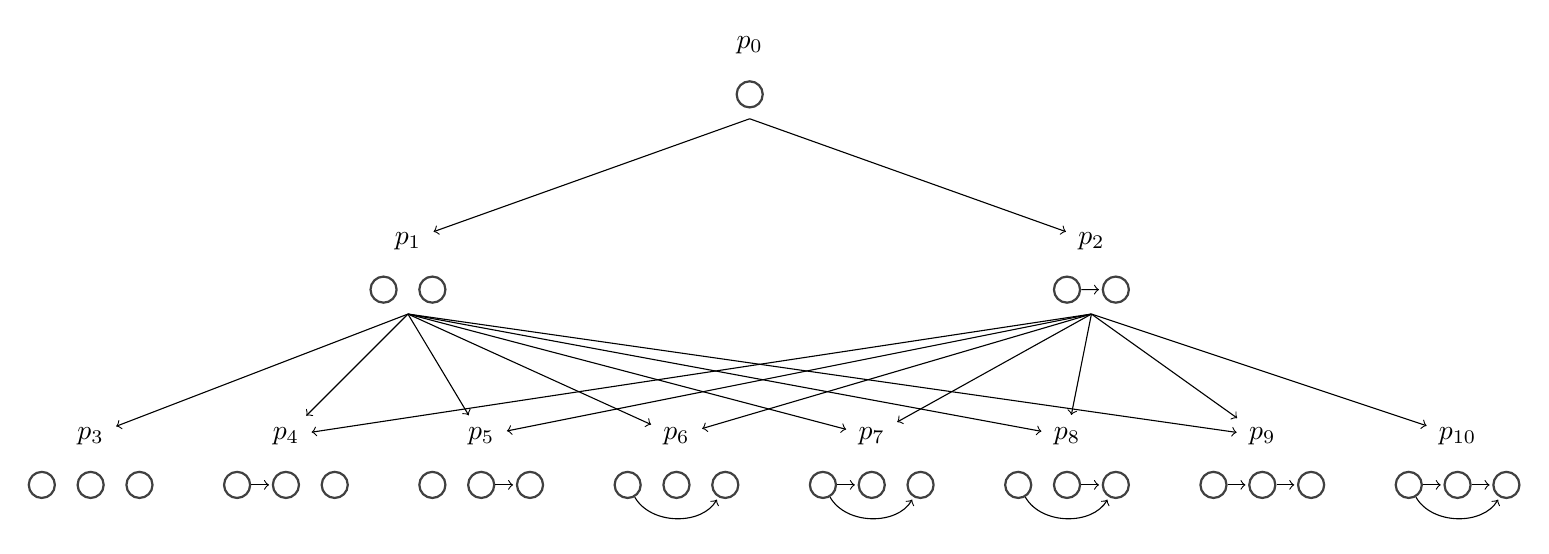
\begin{tikzpicture}[shorten >=1pt,->,scale=0.62]

     \tikzstyle{node}=[circle,thick,draw=black!75,minimum size=1mm]
      
      \begin{scope} 
         \node[node] (p31) at (0,0) {}; 
         \node[node] (p32) at (1,0) {}; 
         \node[node] (p33) at (2,0) {}; 


         \node[node] (p41) at (4,0) {}; 
         \node[node] (p42) at (5,0) {}; 
         \node[node] (p43) at (6,0) {}; 
         \draw[->] (p41) to (p42) ;

         \node[node] (p51) at (8,0) {}; 
         \node[node] (p52) at (9,0) {}; 
         \node[node] (p53) at (10,0) {}; 
         \draw[->] (p52) to (p53) ;

         \node[node] (p61) at (12,0) {}; 
         \node[node] (p62) at (13,0) {}; 
         \node[node] (p63) at (14,0) {}; 
         \draw[->, bend right=60] (p61) to (p63) ;

         \node[node] (p71) at (16,0) {}; 
         \node[node] (p72) at (17,0) {}; 
         \node[node] (p73) at (18,0) {}; 
         \draw[->] (p71) to (p72);
         \draw[->, bend right=60] (p71) to (p73);

         \node[node] (p81) at (20,0) {}; 
         \node[node] (p82) at (21,0) {}; 
         \node[node] (p83) at (22,0) {}; 
         \draw[->] (p82) to (p83);
         \draw[->, bend right=60] (p81) to (p83);

         \node[node] (p91) at (24,0) {}; 
         \node[node] (p92) at (25,0) {}; 
         \node[node] (p93) at (26,0) {}; 
         \draw[->] (p91) to (p92);
         \draw[->] (p92) to (p93);

         \node[node] (p101) at (28,0) {}; 
         \node[node] (p102) at (29,0) {}; 
         \node[node] (p103) at (30,0) {}; 
         \draw[->] (p101) to (p102);
         \draw[->] (p102) to (p103);
         \draw[->, bend right=60] (p101) to (p103);


         \node (p3) at (1,1) {$\tiny{p_3}$};
         \node (p4) at (5,1) {$\tiny{p_4}$};
         \node (p5) at (9,1) {$\tiny{p_5}$};
         \node (p6) at (13,1) {$\tiny{p_6}$};
         \node (p7) at (17,1) {$\tiny{p_7}$};
         \node (p8) at (21,1) {$\tiny{p_8}$};
         \node (p9) at (25,1) {$\tiny{p_9}$};
         \node (p10) at (29,1) {$\tiny{p_{10}}$};

         \node[node] (p11) at (7,4) {}; 
         \node[node] (p12) at (8,4) {}; 

         \node[node] (p21) at (21,4) {}; 
         \node[node] (p22) at (22,4) {}; 
         \draw[->] (p21) to (p22);

         \node (p1) at (7.5,5) {$\tiny{p_1}$};
         \node (p2) at (21.5,5) {$\tiny{p_2}$}; 

         \node[node] (p01) at (14.5,8) {};

         \node (p0) at (14.5,9) {$\tiny{p_0}$};

         \draw[->] (14.5,7.5) to (p1);
         \draw[->] (14.5,7.5) to (p2);
         \draw[->] (7.5,3.5) to (p3);
         \draw[->] (7.5,3.5) to (p4);
         \draw[->] (7.5,3.5) to (p5);
         \draw[->] (7.5,3.5) to (p6);
         \draw[->] (7.5,3.5) to (p7);
         \draw[->] (7.5,3.5) to (p8);
         \draw[->] (7.5,3.5) to (p9);

         
         \draw[->] (21.5,3.5) to (p4);
         \draw[->] (21.5,3.5) to (p5);
         \draw[->] (21.5,3.5) to (p6);
         \draw[->] (21.5,3.5) to (p7);
         \draw[->] (21.5,3.5) to (p8);
         \draw[->] (21.5,3.5) to (p9);
         \draw[->] (21.5,3.5) to (p10);

      \end{scope}        
  \end{tikzpicture}
  }
\end{center}
\caption{hierarchical relations among patterns.} 
\label{fig:parent_child_rel}
\end{figure*}


The weight of a connection from pattern $p_i$ to pattern $p_j$ is the frequency of pattern $p_i$ as a subgraph in pattern $p_j$:

\begin{equation*}
w_{ij} = \frac{count(p_i, p_j)}{\sum_{p_l \in A}count(p_i,p_l)},
\end{equation*}
%
where $A$ is all patterns with \knode\ and $k$ equals the number of nodes of $p_j$. 
In other words, weight $w_{ij}$ is the normalized count of $p_i$ in $p_j$ with respect to all children of (i.e.\ outgoing edges from) $p_i$. 
We use this weighted hierarchical relations between patterns to compute base probabilities of patterns. 
The base probability of pattern $p_j$ is the inner product
of the \mbox{Kneser-Ney} probabilities of its parents considering the weights of their relations with $p_j$:

\begin{equation*}
P_b(p_j)  = P \cdot W,
\end{equation*}
%
where $P$ is a vector of \mbox{Kneser-Ney} probabilities of all patterns that are parents of $p_j$ and $W$ is the weight vector of relations between them. 

This method of smoothing recursively traverse the tree bottom-up, i.e., from large subgraphs to small subgraphs. 
We assume that the probability of the parent of $p_0$ is one because its parent is a graph with no nodes that is a subgraph of any graph.
Because the edge weights are in the range $[0,1]$ the
sum of the probabilities of all patterns with \knode\ is always
equal to one. 

\paragraph{Proof.} 
Assume $I$ and $J$ are the set of all \knode\ and \kplusnode\
patterns where $I$ has $N$ patterns and $J$ has $M$ patterns. 
We prove that if $\sum_{i=1}^N p(p_i)=1$ then 
\begin{equation*}
\sum_{j=1}^M p(p_j)=1. 
\end{equation*}
%
We start to compute the sum of probabilities of all patterns in level $J$, which is: 
\begin{equation*}
\sum_{j=1}^M p(sg_j).
\end{equation*}
%
Based on the definition of base probability, the value of
$p(p_j)$ is computed based on its parents in $I$,

\begin{equation*}
p(p_j)=\sum_{i=1}^N w_{ij}p(p_i),
\end{equation*}
%
where $w_{ij}$ is the weight of the \mbox{parent-child} relation between
$p_i$ and $p_j$. 
Now we have:

\begin{equation*}\sum_{j=1}^M p(p_j) = \sum_{j=1}^M\sum_{i=1}^N w_{ij}p(p_i).
\end{equation*}
%
If we exchange the place of the sums and \mbox{re-write} the equation, we have: 

\begin{equation*}
\sum_{j=1}^M p(p_j) = \sum_{i=1}^N \sum_{j=1}^M w_{ij}p(p_i).
\end{equation*}
%
In this equation $p(p_i)$ is independent of $j$ (index of the inner sum), so it can be moved out of the inner sum:

\begin{equation*}
\sum_{j=1}^M p(p_j) = \sum_{i=1}^N p(p_i) \sum_{j=1}^M w_{ij}
\end{equation*}
%
The inner sum equals $1$ because weights are normalized. 
Therefore we have:

\begin{equation*}
\sum_{j=1}^m p(sg_j) = \sum_{i=1}^n p(sg_i).
\end{equation*}
%
Based on our assumption that sum of probabilities of patterns in level $I$ of the tree is $1$, the right side of the equation is $1$ and 

\begin{equation*}
\sum_{j=1}^m p(sg_j) = 1.
\end{equation*}
%
Therefore, the sum of the base probabilities of all \kplusnode\ subgraphs is $1$. \QEDB



\section{Experiments: Readability Assessment}
\label{sec:experiments}
In this chapter, we evaluate our lexical cohesion graph model on the readability assessment task. 
Similar to the previous chapter we approach readability assessment as the task of ranking texts with respect to their readability. 
The intuition is that more coherent texts are easier to
read. 


\subsection{Data}
We run our experiments on two datasets whose texts are annotated with readability information by human annotators.
The first dataset is the one that we employed in the previous chapter: \pitlerds\ \cite{pitler08}. 
It contains $27$ news articles that are randomly selected from
the Wall Street Journal corpus. 
%
% \footnote{\newcite{pitler08}'s dataset contains 30 articles. They
%   remove one. We assume this is \texttt{wsj\--0382} which
% does not exist in the Penn Treebank. We furthermore remove
% \texttt{wsj\--2090} which does not exist in the final release of the
% Penn Discourse Treebank. We also remove \texttt{wsj\--1398} which is a
% poem and, hence, not very informative for readability assessment.}. 
The average number of sentences is about $10$ words. 
Every article is associated with a human score between $[0.0,5.0]$ indicating the readability score of that article. 
We create pairs of documents, if the difference between their readability scores is greater than $0.5$. 
If the first document in a pair has the higher score, we label
this pair with $+1$, otherwise with $-1$. 
The resulting number of text pairs in this dataset is $209$.

The second dataset is the \declercqds\ dataset that consists of $105$ articles from four different genres: 
\begin{itemize}
  \item  administrative (17 articles), 
  \item  journalistic (43 articles), 
  \item manuals (14 articles)
  \item miscellaneous (31 articles). 
\end{itemize}

The average number of sentences is about $12$. 
This dataset was annotated by \newcite{declercq14} by asking human judges to compare two texts with respect to their readability. 
They use five labels:

\squishlist
\item[\textbf{LME:}] left text is much easier,
\item[\textbf{LSE:}] left text is somewhat easier, 
\item[\textbf{ED:}] both texts are equally difficult,
\item[\textbf{RSE:}] right text is somewhat easier,
\item[\textbf{RME:}] right text is much easier.
\squishend

We map these labels to three class labels $\lbrace -1, 0, +1 \rbrace$, where $+1$ is the label of text pairs that left text is easier to read (LME or LSE); $0$ is for text pairs where both texts are equally difficult to read (ED); and  $-1$ is for text pairs where the right text is easier to read (RSE or RME). 
Table \ref{table:genre_prop} summarizes some properties of this dataset.

\begin{table}[!h]
\centering
\begin{tabular}{lcc}
\hline
Genre & No.\ of articles & No.\ of text pairs \\\hline
Administrative & 17 & 272 \\
Journalistic & 43 & 1806 \\
Manuals & 14 & 182 \\
Miscellaneous & 31 & 931\\\hline
\end{tabular}
\caption{Properties of the different genres in the \emph{De Clercq} dataset.}
\label{table:genre_prop}
\end{table}

\subsection{Experimental Settings}
\paragraph{Word Embeddings and Classification.} In order to reduce the effect of very frequent words, stop words are filtered by using the SMART English stop word list \cite{salton71}. 
We use GloVe as \mbox{pre-trained} word embeddings, which is provided by Stanford. 
Word embeddings are trained on Common Crawl with 840B tokens, 2.2M vocabulary. 
We represent each word by a vector with length 300 \cite{pennington14}. 
For handling \mbox{out-of-vocabulary} words, we assign a random vector to each word and memorize it for its next occurrence \cite{kusner15}. 
The classification task is performed by the Support Vector Machine (SVM) implementation in WEKA (SMO) with the linear kernel function.  
All settings are set to the default values. 
The evaluation is computed by \mbox{10-fold} \mbox{cross-validation}. 

\paragraph{Graph Processing and Smoothing.} In order to compare the performance of LCG with the entity graph model, we follow
our settings in previous chapter and use the gSpan method \cite{yanxifeng02} to extract subgraphs that are occurring in graph representations of documents in a corpus and compute their frequencies. 
Note that gSpan does not extract all possible \knode\ subgraphs, whereas for applying the \mbox{Kneser-Ney} smoothing we need to  to count all possible \knode\ subgraphs, because the probability should be distributed among all possible subgraphs.  
This also helps to estimate the probability of unseen patterns. 
So in the experiments that we use smoothing, we compute the frequencies of coherence patterns by the sampling method that is explained in this chapter.  
In this regard, we take $10,000$ samples of the given sentence graph. 
We compute the base probability for at most $k = 6$. 
We find the best value for $d$ in a greedy manner. 
First, we initialize $\alpha$ with $0.001$. 
In each iteration we compute the performance. 
Then we multiply the discount factor by $10$. 
We iterate as long as the discount factor is less than $1000$. We report the best performance.
We filter out edges of a lexical graph if their cosine similarity is less than threshold $0.9$
We selected $0.9$ to connect only sentences with high confidence. 
We selected this value to ensure that we are not adding noise to our graphs by considering weak relations.  
we extend the \emph{EGrid} model by a pronoun resolution system, so that entities mentioned by pronouns also enter the graph. 
We apply the Stanford coreference resolution system \cite{leeheeyoung13}. 
Using the full coreference resolution system, however, decreases performance, hence we only use resolved pronouns.



\subsubsection{Results}
First we evaluate our the lexical graph representation on the  \pitlerds\ dataset. 
We use the majority class baseline (\emph{ZeroR}) classifier to put our results into context. 
Our second baseline is \emph{EGrid} \cite{barzilay08} which we use as non-trivial baseline.   
Table \ref{table:pitler_dataset} reports the accuracy of \emph{LCG}\ with different values for $k$ in \knode\ subgraphs for coherence pattern mining. 
For sake of fairness, in all examined models in this experiment we use gSpan for extracting and counting patterns in graphs. 

\begin{table}[!ht]
\begin{center}
\begin{tabular}{lcc}
\hline
System  & \multicolumn{2}{c}{Accuracy}\\
\hline
ZeroR   & \multicolumn{2}{c}{50.24\%}\\
EGrid   & \multicolumn{2}{c}{83.25\%}\\
\hline
\knode\ & EGraph+PRN &  LCG        \\
\hline
3-node  &    80.38\%   &  78.95\%  \\
4-node  &    89.95\%   &  89.47\%  \\
5-node  &    95.69\%   &  97.13\%  \\
\hline
\end{tabular}
\end{center}
\caption{Results on the \pitlerds\ dataset.}
\label{table:pitler_dataset}
\end{table}

When \emph{3-node}\ coherence patterns are employed as coherence patterns, the lexical coherence graph model, \emph{LCG}, performs slightly worse than \emph{EGraph}.  
This is because graphs in the \emph{LCG}\ model have more edges than graphs in
\emph{EGraph}. 
When graphs become denser, \emph{3-node}\ patterns occur in every graph and therfore their frequency is less discriminative.  
This is much clearer when we increase the size of subgraphs to capture more information about the connectivity style of graphs. 
By increasing the size of coherence patterns from \emph{3-nodes} to \emph{4-nodes}, we see that the performance of \emph{LCG} is on par with the \emph{EGraph} model. 
The difference between the accuracies of the two systems is diminished because \emph{4-node} patterns contain more edges than 3-node subgraphs. 
They capture the connectivity style of denser graphs better. 
Finally, when we use 5-node coherence patterns the LCG model significantly ($p\_value=0.01$) outperforms the EGraph model leading to this result that our lexical coherence graph is a better representative of sentence relations for coherence modeling than the entity graph model, if sufficiently large subgraphs are employed.  

Beside the above observations, results in Table \ref{table:pitler_dataset} show that both the entity graph model and the LCG model capture coherence better than the EGrid model \cite{barzilay08}.  
It is because graph-based models take long distant relations between sentences into account, which is informative for coherence modeling.  
Results in Table \ref{table:pitler_dataset} also depict that the accuracy of both LCG and EGraph models increases by increasing the size of patterns. 
This is compatible with results of the previous chapter, and confirms our intuition that larger subgraphs have more capacity to capture the connectivity style of graph representations of texts and therefore are better patterns for coherence modeling. 
The difference between \emph{LCG} and \emph{EGraph} using 4-node subgraphs is not significant.

Table \ref{table:clercq} shows the performance of different models on the \declercqds dataset.  

\begin{table}[!ht]
\centering
\begin{tabular}{lccc}
\hline
System & \multicolumn{2}{c}{Accuracy}   \\
\hline  
ZeroR	& \multicolumn{2}{c}{$42.312$\%}    \\\hline
\knode\ & EGraph	& LCG\textsuperscript{$\twowhitestars$}     \\\hline

3-node & $42.31\%$ & $42.31\%^\twowhitestars$       \\
4-node & $48.07\%$ & $49.12\%^\twostars$             \\
5-node & $65.77\%$ & $76.27\%^\twostars$	           \\\hline

\end{tabular}
\caption{Results on the \declercqds\ dataset.}
\label{table:clercq}
\end{table}

We use a majority baseline (\emph{ZeroR}) to put our results in context. 
The performance of both EGraph and LCG methods is on par with the baseline for \emph{3-node}\ patterns. 
\emph{4-node} patterns work already better than the baseline, and \emph{5-node}\ patterns yield reasonable performance on the \declercqds dataset. 

The general performance on the \declercqds dataset is lower than the performance on the \pitlerds dataset. 
The main reason for this can be that texts in the \declercqds dataset are from four different genres and coherence patterns may vary across genres. 
% first, text-pairs in the \declercqds dataset are associated with a label from three classes whereas the labels of text-pairs in the \pitelerds dataset are from binary classes.  
% Three-label classification is more difficult than the binary classification task. 
% Second, texts in the \declercq dataset are from four different genres and coherence patterns
% may vary across genres. 
In order to gain an insight to this, we compute the performance of these systems on texts exclusively from each genre in the \declercqds dataset. 

\begin{table}[!ht]
\centering
\begin{tabular}{lccc}
\hline
\emph{5-node}\  & EGraph      & LCG       \\\hline
Administrative	& $69.49\%$	  & $71.69\%$	\\
Journalistic	  & $65.01\%$	  & $82.12\%$ \\
Manuals 		    & $54.95\%$ 	& $61.54\%$	\\
Misc.			      & $70.68\%$	  & $76.69\%$ \\\hline
\end{tabular}
\caption{Accuracy of \emph{EGraph}\ and \emph{LCG}\ on different
  genres in the \declercqds dataset.}
\label{table:declercq_genre}
\end{table}

Table \ref{table:declercq_genre} shows the performance for \emph{EGraph}\ and \emph{LCG}\ using \emph{5-node}\ patterns on different genres in the \declercqds dataset. 
The performance of \emph{LCG}\ is better than \emph{EGraph}\ on all genres. 
Unlike \emph{EGraph}, \emph{LCG}\ gets the best performance on journalistic articles. 
The lowest performance of both models is obtained on manuals. 

\textbf{TODO: What is in this genres that make your model work better?}

While large subgraphs are very informative for coherence modeling (especially for dense graphs as shown in Table \ref{table:clercq}), many large subgraphs $k>5$ have low or zero frequency in a graph.
This yields a sparsity problem. 
On the other hand, large subgraphs occur in few graphs in a dataset. 
So when large subgraphs are taken into account, each graph is represented by a large vector, because there are many possible large subgraphs, where most of its elements are zero.   
The problem with such vectors is that each graph representation becomes unique in a dataset and a machine learning model cannot learn from similarity and dissimilarity between graphs. 
In practice, we observe a drop in performance when the model deals with large subgraphs (\emph{6-node} subgraphs, \emph{LCG1}\ for \emph{P\&N}\ in Table \ref{table:smoothing}). 

We solve this problem by our adapted version of \mbox{Kneser-Ney} smoothing. 
To do this, we use our proposed sampling method in Section \ref{} to count all possible (connected and disconnected) \knode\ subgraphs. 

Table \ref{table:smoothing} shows the performance of the \emph{LCG}\ model where the sampling method is employed for counting patterns with different number of nodes. 
It also shows the result of smoothing method in different columns. 
The performance on the \pitlerds dataset suddenly drops for \emph{6-node}\ subgraphs. 
This is because of the sparsity problem. 

\textbf[TODO: can you say what percentage of frequencies are zero in 6-node patterns and 5-node patterns? ]


\begin{table}[!ht]
\begin{center}
\begin{tabular}{ccccc}
\hline
 & \multicolumn{2}{@{}c}{\pitlerds}  & \multicolumn{2}{c@{}}{\declercqds} \\
 \hline
\knode\ & -- Smoothing & + Smoothing & -- Smoothing & + Smoothing \\\hline
3-node &     $84.52\%$ & $89.00\%$   & $42.31\%$    &   $49.60\%$ \\
4-node &     $95.69\%$ & $96.17\%$   & $65.10\%$    &   $66.23\%$ \\
5-node &     $97.61\%$ & $98.08\%$   & $79.33\%$    &   $79.85\%$ \\
6-node &     $93.26\%$ & $95.69\%$   & $76.67\%$    &   $78.03\%$\\
\hline
\end{tabular}
\end{center}
\caption{Applying smoothing method on the LCG model yields to higher accuracies for larger subgraphs.}
\label{table:smoothing}
\end{table}

When we apply the \mbox{Kneser-Ney} smoothing, as described in Section \ref{}, the results for all examined values of $k$ are improved for both datasets (Table \ref{table:smoothing}).

Interestingly, \mbox{Kneser-Ney} smoothing improves the performance of the system even with \emph{3-node}\ subgraphs by a large margin. 
Smoothing reduces the power of frequency and makes the frequency distribution of subgraphs more even. 
It decreases the effect of frequency through alls subgraphs by considering parent-child relations between subgraphs to relate similar subgraphs. 
That is the advantage of the \mbox{Kneser-Ney} method in comparison to the other smoothing methods like
Laplace \cite{}. 

On the \emph{P\&N}\ dataset, we achieve the best results to date. 
\newcite{pitler08} reported 83.25\% accuracy, \newcite{mesgar15} 89.95\%. 
When smoothing \emph{5-node}\ subgraphs we are able to report 98.08\%. 
This, however, indicates that this dataset may not be the best one to report performance on and evaluate our coherence model. 
Hence, we check if smoothing also improves the performance on the more difficult \declercqds dataset.
On the \declercqds dataset, we basically observe the same trends. 
Both settings result in better performance than \emph{LCG}\ (see Table \ref{table:clercq}) confirming that our sampling model is as powerful as the normal counting but more computationally efficient.  

Note that none of the parameters (such the maximum number samples drawn from a graph and the threshold for filtering edges of the LCG graph) in this work is tuned on the datasets. 
One may get better performance by tuning the parameters.

\textbf{[TO DO: any report about the effect of the treshold on results?]}

To summarize this part, the results confirm the intuition that the lexical coherence graph \emph{LCG}\ captures coherence and models lexical cohesion appropriately.
Applying smoothing on graphs of \emph{EGraph} model increases the performance of this model. 
But this improvement is not as high as the obtained improvement on the \emph{LCG} graph.
This shows that our smoothing method is useful for both graph-based models, and our new graph representation is more informative than the entity graph model for coherence modeling. 

\paragraph{Coherence Patterns.}
In this part we compute the Pearson correlation coefficient between the frequency of a few patterns in the lexical coherence graphs of texts in the \emph{P\&N}\ dataset and the ratings of texts which are assigned by humans. 

Among all \emph{3-node}\ patterns only the frequency of one pattern in the lexical coherence graphs is significantly and positively correlated (\emph{p-value}$<0.05$) with human readability scores. 
This graph is shown in Figure \ref{fig:correlated_graphs}. 
Among the patterns with four nodes, frequencies of six patterns are significantly correlated with readability scores assigned by humans. 
Only one is positively correlated, while five are negatively correlated. 
Interestingly, both positively correlated \emph{3-node}\ and \emph{4-node}\ subgraphs have been determined as positively and significantly correlated with human readability scores in Chapter \ref{}. 

\begin{figure}[!ht]
\centering
\begin{tabular}{lc|cc}
\hline
& Pattern & $\rho$ & p-value \\
\hline
%%%%%%%%%%%%%%%%%%%%%%%%%%%%%%%%%%%%%%%%%%%%%%%%%%%%
\rb{\emph{3-node}} &
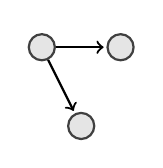
\begin{tikzpicture}[shorten >=1pt,->,scale=0.5]  
        \tikzstyle{sentence}=[circle,thick,draw=black!75,fill=black!10,minimum size=2mm]
        \tikzstyle{edge}=[draw, thick]
       \begin{scope}
         \node [sentence] (s1) at (0,2) {\tiny{}};
         \node [sentence] (s2) at (2,2) {\tiny{}};
         \node [sentence] (s3) at (1,0) {\tiny{}}; 
         \path[edge] (s1) edge [above] node[font=\tiny] {} (s2);
         \path[edge] (s1) edge [above] node[font=\tiny] {} (s3);
        \end{scope}        
\end{tikzpicture}
      & \rb{0.43} & \rb{0.024}
      \\\hline
\rb{\emph{4-node}} &
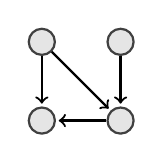
\begin{tikzpicture}[shorten >=1pt,->,scale=0.5]  
        \tikzstyle{sentence}=[circle,thick,draw=black!75,fill=black!10,minimum size=1mm]
        \tikzstyle{edge}=[draw, thick]
       \begin{scope}
         \node [sentence] (s1) at (0,2) {\tiny{}};
         \node [sentence] (s2) at (2,2) {\tiny{}};
         \node [sentence] (s3) at (2,0) {\tiny{}};
         \node [sentence] (s4) at (0,0) {\tiny{}};  
         \path[edge] (s1) edge [above] node[font=\tiny] {} (s3);
         \path[edge] (s1) edge [above] node[font=\tiny] {} (s4);
         \path[edge] (s2) edge [above] node[font=\tiny] {} (s3);
         \path[edge] (s3) edge [above] node[font=\tiny] {} (s4);
        \end{scope}        
      \end{tikzpicture}
      & \rb{-0.45} & \rb{0.018}
      
       \\
&
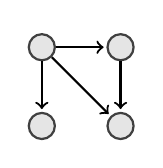
\begin{tikzpicture}[shorten >=1pt,->,scale=0.5]  
        \tikzstyle{sentence}=[circle,thick,draw=black!75,fill=black!10,minimum size=1mm]
        \tikzstyle{edge}=[draw, thick]
       \begin{scope}
         \node [sentence] (s1) at (0,2) {\tiny{}};
         \node [sentence] (s2) at (2,2) {\tiny{}};
         \node [sentence] (s3) at (2,0) {\tiny{}};
         \node [sentence] (s4) at (0,0) {\tiny{}};  
         \path[edge] (s1) edge [above] node[font=\tiny] {} (s2);
         \path[edge] (s1) edge [above] node[font=\tiny] {} (s3);
         \path[edge] (s1) edge [above] node[font=\tiny] {} (s4);
         \path[edge] (s2) edge [above] node[font=\tiny] {} (s3);
        \end{scope}        
      \end{tikzpicture}
      & \rb{+0.39} & \rb{0.047}
      \\
&
      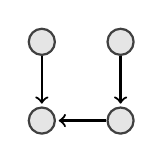
\begin{tikzpicture}[shorten >=1pt,->,scale=0.5]  
        \tikzstyle{sentence}=[circle,thick,draw=black!75,fill=black!10,minimum size=1mm]
        \tikzstyle{edge}=[draw, thick]
       \begin{scope}
         \node [sentence] (s1) at (0,2) {\tiny{}};
         \node [sentence] (s2) at (2,2) {\tiny{}};
         \node [sentence] (s3) at (2,0) {\tiny{}};
         \node [sentence] (s4) at (0,0) {\tiny{}};  
         \path[edge] (s1) edge [above] node[font=\tiny] {} (s4);
         \path[edge] (s2) edge [above] node[font=\tiny] {} (s3);
         \path[edge] (s3) edge [above] node[font=\tiny] {} (s4);
        \end{scope}        
      \end{tikzpicture}
      &  \rb{-0.43}  & \rb{0.024}
      \\
&
      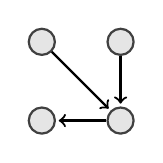
\begin{tikzpicture}[shorten >=1pt,->,scale=0.5]  
        \tikzstyle{sentence}=[circle,thick,draw=black!75,fill=black!10,minimum size=1mm]
        \tikzstyle{edge}=[draw, thick]
       \begin{scope}
         \node [sentence] (s1) at (0,2) {\tiny{}};
         \node [sentence] (s2) at (2,2) {\tiny{}};
         \node [sentence] (s3) at (2,0) {\tiny{}};
         \node [sentence] (s4) at (0,0) {\tiny{}};  
         \path[edge] (s1) edge [above] node[font=\tiny] {} (s3);
         \path[edge] (s2) edge [above] node[font=\tiny] {} (s3);
         \path[edge] (s3) edge [above] node[font=\tiny] {} (s4);
        \end{scope}        
      \end{tikzpicture}
      & \rb{-0.59} & \rb{0.001}
      \\
&
      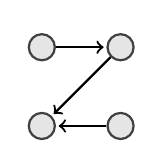
\begin{tikzpicture}[shorten >=1pt,->,scale=0.5]  
        \tikzstyle{sentence}=[circle,thick,draw=black!75,fill=black!10,minimum size=1mm]
        \tikzstyle{edge}=[draw, thick]
       \begin{scope}
         \node [sentence] (s1) at (0,2) {\tiny{}};
         \node [sentence] (s2) at (2,2) {\tiny{}};
         \node [sentence] (s3) at (2,0) {\tiny{}};
         \node [sentence] (s4) at (0,0) {\tiny{}};  
         \path[edge] (s1) edge [above] node[font=\tiny] {} (s2);
         \path[edge] (s2) edge [above] node[font=\tiny] {} (s4);
         \path[edge] (s3) edge [above] node[font=\tiny] {} (s4);
        \end{scope}        
      \end{tikzpicture}
      & \rb{-0.55} & \rb{0.003}
      \\
&
      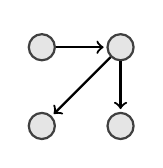
\begin{tikzpicture}[shorten >=1pt,->,scale=0.5]  
        \tikzstyle{sentence}=[circle,thick,draw=black!75,fill=black!10,minimum size=1mm]
        \tikzstyle{edge}=[draw, thick]
       \begin{scope}
         \node [sentence] (s1) at (0,2) {\tiny{}};
         \node [sentence] (s2) at (2,2) {\tiny{}};
         \node [sentence] (s3) at (2,0) {\tiny{}};
         \node [sentence] (s4) at (0,0) {\tiny{}};  
         \path[edge] (s1) edge [above] node[font=\tiny] {} (s2);
         \path[edge] (s2) edge [above] node[font=\tiny] {} (s3);
         \path[edge] (s2) edge [above] node[font=\tiny] {} (s4);
        \end{scope}        
      \end{tikzpicture}
      & \rb{-0.55} & \rb{0.003}\\
      \hline
      
\end{tabular}
\caption{Pearson correlation coefficient between \emph{3-node}\ and \emph{4-node}\
  subgraphs and readability scores in the \emph{P\&N}\ dataset.}
\label{fig:correlated_graphs}
\end{figure}


\section{Conclusions}
\label{sec:lcg_conclusion}
%
In this chapter we proposed a new graph based coherence model, the lexical coherence graph, LCG. 
We view coherence as semantic connectedness between words which we model by word embeddings. 
We take only the strongest connection between sentences to create a graph with connected sentences. 
Then we extract large subgraphs capturing coherence patterns, which show similarity to patterns described in
text linguistics \cite{danes74a}.

While the entity grid works only on sequences of up to two adjacent sentences, we are able to model relationships of up to six non-adjacent sentences. 
We solve the sparsity problem of large subgraphs by adapting \mbox{Kneser-Ney} smoothing to graphs. 
Smoothing prevents LCG from losing performance with large subgraphs and leads to superior performance on the \newcite{pitler08} dataset and to a first reasonable \mbox{state-of-the-art} on the \newcite{declercq14} dataset.
